\documentclass[aspectratio=43]{beamer}

\usetheme{Boadilla}
\setbeamertemplate{footline}[page number]{}
\setbeamertemplate{navigation symbols}{}

\usepackage{times}
\usepackage{tikz}
\usefonttheme{structurebold}
\usepackage{listings}

% Suppress the navigation bar
\beamertemplatenavigationsymbolsempty

\newenvironment{changemargin}[1]{% 
  \begin{list}{}{% 
    \setlength{\topsep}{0pt}% 
    \setlength{\leftmargin}{#1}% 
    \setlength{\rightmargin}{1em}
    \setlength{\listparindent}{\parindent}% 
    \setlength{\itemindent}{\parindent}% 
    \setlength{\parsep}{\parskip}% 
  }% 
  \item[]}{\end{list}} 

\title{Lecture 02---Amdahl's Law, Modern Hardware}
\subtitle{ECE 459: Programming for Performance}
\author{Patrick Lam}
\institute{University of Waterloo}
\date{January 7, 2015}

\begin{document}

%%%%%%%%%%%%%%%%%%%%%%%%%%%%%%%%%%%%%%%%%%%%%%%%%%%%%%%%%%%%%%%%%%%%%%%%%%%%%%%%
\begin{frame}[plain]
  \titlepage
\end{frame}
%%%%%%%%%%%%%%%%%%%%%%%%%%%%%%%%%%%%%%%%%%%%%%%%%%%%%%%%%%%%%%%%%%%%%%%%%%%%%%%%

%%%%%%%%%%%%%%%%%%%%%%%%%%%%%%%%%%%%%%%%%%%%%%%%%%%%%%%%%%%%%%%%%%%%%%%%%%%%%%%%
\begin{frame}
  \frametitle{About Prediction and Speedups}

\begin{center}
Cliff Click said: ``5\% miss rates dominate performance.'' \\[2em]

Why is that?\\[2em]
\only<2>{Recall: 100-1000 slot penalty for a miss.\\[1em]}
\only<2>{See {\tt L02.pdf} for a calculation.}
\end{center}
\end{frame}
%%%%%%%%%%%%%%%%%%%%%%%%%%%%%%%%%%%%%%%%%%%%%%%%%%%%%%%%%%%%%%%%%%%%%%%%%%%%%%%%

%%%%%%%%%%%%%%%%%%%%%%%%%%%%%%%%%%%%%%%%%%%%%%%%%%%%%%%%%%%%%%%%%%%%%%%%%%%%%%%%
\begin{frame}[fragile]
  \frametitle{Forcing Branch Mispredicts}

\begin{center}
\url{blog.man7.org/2012/10/how-much-do-builtinexpect-likely-and.html}
\end{center}

{\tiny
\begin{verbatim}
#include <stdlib.h>
#include <stdio.h>

static __attribute__ ((noinline)) int f(int a) { return a; }

#define BSIZE 1000000
int main(int argc, char* argv[]) 
{
  int *p = calloc(BSIZE, sizeof(int));
  int j, k, m1 = 0, m2 = 0;
  for (j = 0; j < 1000; j++) {
    for (k = 0; k < BSIZE; k++) {
      if (__builtin_expect(p[k], EXPECT_RESULT)) {
        m1 = f(++m1);
      } else {
        m2 = f(++m2);
      }
    }
  }

  printf("%d, %d\n", m1, m2);
}
\end{verbatim}
}
Running times: 3.1s with good (or no) hint, 4.9s with bogus hint.
\end{frame}
%%%%%%%%%%%%%%%%%%%%%%%%%%%%%%%%%%%%%%%%%%%%%%%%%%%%%%%%%%%%%%%%%%%%%%%%%%%%%%%%

%%%%%%%%%%%%%%%%%%%%%%%%%%%%%%%%%%%%%%%%%%%%%%%%%%%%%%%%%%%%%%%%%%%%%%%%%%%%%%%%
\begin{frame}
  \frametitle{Limitations of Speedups}
\hspace*{.2\textwidth}\begin{minipage}{.75\textwidth}
    Our main focus is parallelization.\\[1em]
  \begin{itemize}
    \vfill
    \item Most programs have a sequential part and a parallel part; and,\\[1em]
    \item Amdahl's Law answers, ``what are the limits to parallelization?''
  \end{itemize}
\end{minipage}

\end{frame}
%%%%%%%%%%%%%%%%%%%%%%%%%%%%%%%%%%%%%%%%%%%%%%%%%%%%%%%%%%%%%%%%%%%%%%%%%%%%%%%%

%% intro here

\section{Amdahl's Law}
%%%%%%%%%%%%%%%%%%%%%%%%%%%%%%%%%%%%%%%%%%%%%%%%%%%%%%%%%%%%%%%%%%%%%%%%%%%%%%%%
\begin{frame}
  \frametitle{Formulation (1)}

  \hspace*{2em}\begin{minipage}{.8\textwidth}
  $S$: fraction of serial runtime in a serial execution.

  $P$: fraction of parallel runtime in a serial execution.

  Therefore, $S + P = 1$.\\[2em]

  With 4 processors, best case, what can happen to the following runtime?
  \end{minipage}

  \hspace*{5em}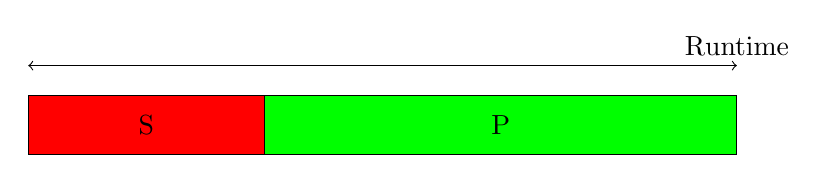
\begin{tikzpicture}
   \draw[<->] (-1.5,0.75) -- (7.5,0.75) node[above] {Runtime};
   \draw (0,0) node[rectangle, fill=red, minimum height=0.75cm, minimum width=3cm,draw] {S};
   \draw (4.5,0) node[rectangle, fill=green, minimum height=0.75cm, minimum width=6cm,draw] {P};
  \end{tikzpicture}
\end{frame}
%%%%%%%%%%%%%%%%%%%%%%%%%%%%%%%%%%%%%%%%%%%%%%%%%%%%%%%%%%%%%%%%%%%%%%%%%%%%%%%%

%%%%%%%%%%%%%%%%%%%%%%%%%%%%%%%%%%%%%%%%%%%%%%%%%%%%%%%%%%%%%%%%%%%%%%%%%%%%%%%%
\begin{frame}
  \frametitle{Formulation (1)}

  \hspace*{5em}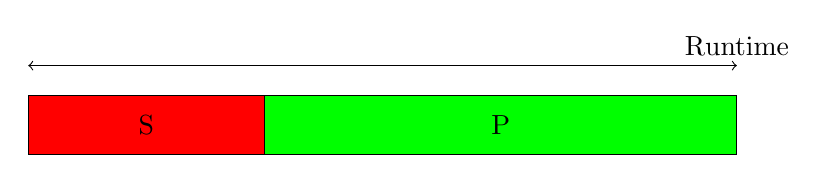
\begin{tikzpicture}
   \draw[<->] (-1.5,0.75) -- (7.5,0.75) node[above] {Runtime};
   \draw (0,0) node[rectangle, fill=red, minimum height=0.75cm, minimum width=3cm,draw] {S};
   \draw (4.5,0) node[rectangle, fill=green, minimum height=0.75cm, minimum width=6cm,draw] {P};
  \end{tikzpicture}
  \vfill
  We want to split up the parallel part over 4 processors
  \vfill
  \hspace*{5em}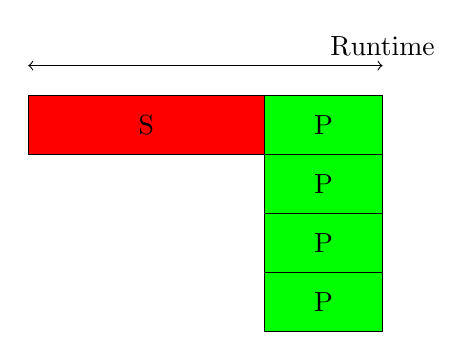
\begin{tikzpicture}
   \draw[<->] (-1.5,0.75) -- (3,0.75) node[above] {Runtime};
   \draw (0,0) node[rectangle, fill=red, minimum height=0.75cm, minimum width=3cm,draw] {S};
   \draw (2.25,0) node[rectangle, fill=green, minimum height=0.75cm, minimum width=1.5cm,draw] {P};
   \draw (2.25,-0.75) node[rectangle, fill=green, minimum height=0.75cm, minimum width=1.5cm,draw] {P};
   \draw (2.25,-1.5) node[rectangle, fill=green, minimum height=0.75cm, minimum width=1.5cm,draw] {P};
   \draw (2.25,-2.25) node[rectangle, fill=green, minimum height=0.75cm, minimum width=1.5cm,draw] {P};
  \end{tikzpicture}
\end{frame}
%%%%%%%%%%%%%%%%%%%%%%%%%%%%%%%%%%%%%%%%%%%%%%%%%%%%%%%%%%%%%%%%%%%%%%%%%%%%%%%%

%%%%%%%%%%%%%%%%%%%%%%%%%%%%%%%%%%%%%%%%%%%%%%%%%%%%%%%%%%%%%%%%%%%%%%%%%%%%%%%%
\begin{frame}
  \frametitle{Formulation (2)}

\Large
$T_s$: time for the program to run in serial

$N$: number of processors/parallel executions

$T_p$: time for the program to run in parallel
\vfill
  \begin{itemize}
    \item Under perfect conditions, get $N$ speedup for $P$
  \end{itemize}
\vfill

  \begin{center}
$T_p = T_s \cdot (S + \frac{P}{N})$
  \end{center}
\end{frame}
%%%%%%%%%%%%%%%%%%%%%%%%%%%%%%%%%%%%%%%%%%%%%%%%%%%%%%%%%%%%%%%%%%%%%%%%%%%%%%%%

%%%%%%%%%%%%%%%%%%%%%%%%%%%%%%%%%%%%%%%%%%%%%%%%%%%%%%%%%%%%%%%%%%%%%%%%%%%%%%%%
\begin{frame}
  \frametitle{Formulation (3)}

  \hspace*{3em} How much faster can we make the program?

  \begin{eqnarray*}
  \mbox{\em speedup} &=& \frac{T_s}{T_p}\\
                     &=& \frac{T_s}{T_S \cdot (S + \frac{P}{N})}\\
                     &=& \frac{1}{S + \frac{P}{N}}
  \end{eqnarray*}
  \vfill
  \hspace*{3em} (assuming no overhead for parallelizing; or costs near
  zero)

\end{frame}
%%%%%%%%%%%%%%%%%%%%%%%%%%%%%%%%%%%%%%%%%%%%%%%%%%%%%%%%%%%%%%%%%%%%%%%%%%%%%%%%

%%%%%%%%%%%%%%%%%%%%%%%%%%%%%%%%%%%%%%%%%%%%%%%%%%%%%%%%%%%%%%%%%%%%%%%%%%%%%%%%
\begin{frame}
  \frametitle{Fixed-Size Problem Scaling, \\ Varying Fraction of Parallel Code}

  \begin{center}
    \hspace*{2em}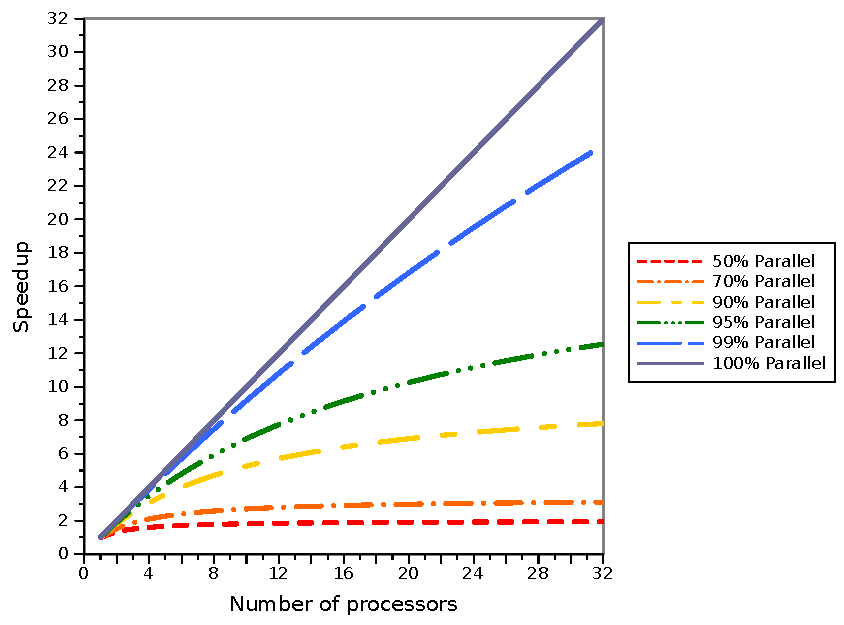
\includegraphics[scale=0.68]{L02/parallel-scaling}
  \end{center}
\end{frame}
%%%%%%%%%%%%%%%%%%%%%%%%%%%%%%%%%%%%%%%%%%%%%%%%%%%%%%%%%%%%%%%%%%%%%%%%%%%%%%%%

%%%%%%%%%%%%%%%%%%%%%%%%%%%%%%%%%%%%%%%%%%%%%%%%%%%%%%%%%%%%%%%%%%%%%%%%%%%%%%%%
\begin{frame}
  \frametitle{Amdahl's Law}

 \hspace*{2em}Replace $S$ with $(1 - P)$:

  \begin{center}
    \structure{$\mbox{\em speedup} = \frac{1}{(1 - P) + \frac{P}{N}}$}
  \end{center}
  \vfill
  \begin{center}
    $\mbox{\em maximum speedup} = \frac{1}{(1 - P)}$, since $\frac{P}{N} \rightarrow 0$
  \end{center}
  \vfill
  \hspace*{2em}\begin{minipage}{.8\textwidth}As you might imagine, the asymptotes in the previous graph are bounded by the
  maximum speedup.\end{minipage}
\end{frame}
%%%%%%%%%%%%%%%%%%%%%%%%%%%%%%%%%%%%%%%%%%%%%%%%%%%%%%%%%%%%%%%%%%%%%%%%%%%%%%%%

% P_estimated
%%%%%%%%%%%%%%%%%%%%%%%%%%%%%%%%%%%%%%%%%%%%%%%%%%%%%%%%%%%%%%%%%%%%%%%%%%%%%%%%
\begin{frame}
  \frametitle{Assumptions behind Amdahl's Law}

  \begin{changemargin}{2cm}
    How can we invalidate Amdahl's Law?
  \end{changemargin}
  
\end{frame}
%%%%%%%%%%%%%%%%%%%%%%%%%%%%%%%%%%%%%%%%%%%%%%%%%%%%%%%%%%%%%%%%%%%%%%%%%%%%%%%%

%%%%%%%%%%%%%%%%%%%%%%%%%%%%%%%%%%%%%%%%%%%%%%%%%%%%%%%%%%%%%%%%%%%%%%%%%%%%%%%%
\begin{frame}
  \frametitle{Assumptions behind Amdahl's Law}

  \begin{changemargin}{2cm}
    We assume:
    \begin{itemize}
    \item problem size is fixed (we'll see this soon);
    \item program/algorithm behaves the same on 1 processor and on $N$ processors; and
    \item that we can accurately measure runtimes---\\ ~~i.e. that overheads don't matter.
    \end{itemize}
  \end{changemargin}
  
\end{frame}
%%%%%%%%%%%%%%%%%%%%%%%%%%%%%%%%%%%%%%%%%%%%%%%%%%%%%%%%%%%%%%%%%%%%%%%%%%%%%%%%


\end{document}
